\documentclass[twocolumn]{summery}
\title{Experimentalphysik III - Zusammenfassung}

\begin{document}
\maketitle
\tableofcontents

\section{Licht}
\subsection{Fermat's Prinzip}
Die geometrische Optik lässt sich mathematisch elegant beschreiben wenn man den Lichtweg 
\(L = \int \abs{\vec r(t)}\cdot n(\vec r (t)) \dt\) definiert. Er ist der normale Weg, gewichtete 
mit dem lokalen Brechungsindex.
Das Licht nimmt immer den Weg, der den Lichtweg extremal werden lässt.
Zur Erinnerung: Es gilt \(n = \frac{c}{v}\)

Es Weg des Lichts kann daher formal mithilfe der Euler-Lagrange Gleichungen beschrieben werden:
\begin{align*}
    \ddt \partiald{\mathcal L}{\vdot x} = \partiald{\mathcal L}{\vec x} \with \mathcal L = \abs{\vec r(t)}\cdot n(\vec r (t))
\end{align*}

\subsection{Snell's Gesetz}
Reist ein Lichtstrahl von einem Medium mit Brechungsindex \(n_1\) in ein zweites mit 
Brechungindex \(n_2\), wird er gebrochen. Der Winkel kann mithilfe von Snell's Gesetz 
berechnet werden:
\begin{align*}
    \frac{\sin\beta}{\sin\alpha} &= \frac{n_a}{n_b}
\end{align*}

\section{Strahlenoptik}
\subsection{Dünne Linsen in Paraxialer Näherung}
Sowohl für Sammel-/ aus auch Streulinsen gelten die Linsengleichungen:
\begin{align*}
    \frac 1g + \frac 1b = \frac 1f
\end{align*}
und 
\begin{align*}
    \frac{b}{g} = \frac BG   
\end{align*}

Linsenmachergleichung für dünne Linsen:
\begin{align*}
    D = \frac {n_0}f &= (n_L - n_0)\hug{\frac 1{r_1} + \frac 1{r_2}}
\end{align*}

Außerdem gilt für dünne Linsen:
\begin{align*}
    D &= D_1 + D_2
\end{align*}

\subsection{Dicke Linsen}
Linsenmachergleichung:
\begin{align*}
    D = \frac {n_0}f &= (n_L - n_0)\hug{\frac 1{r_1} + \frac 1{r_2}}
    + \frac{(n_L - n_0)^2}{n_L}\frac{d}{r_1r_2}
\end{align*}

Newtonsch'sche Abbildungsgleichung
\begin{align*}
    z\cdot z' &= f_B \cdot f_G
\end{align*}

\subsection{Kugelfläche in Paraxialer Näherung}
Für eine Kugelfläche gilt die Abbe'sche Invariante:
\begin{align*}
    n_0 \hug{\frac 1r + \frac 1g} &= n_l \hug {\frac 1r - \frac 1b}
\end{align*}
 
\section{Fotometrie}
\begin{figure}[H]
    \centering
    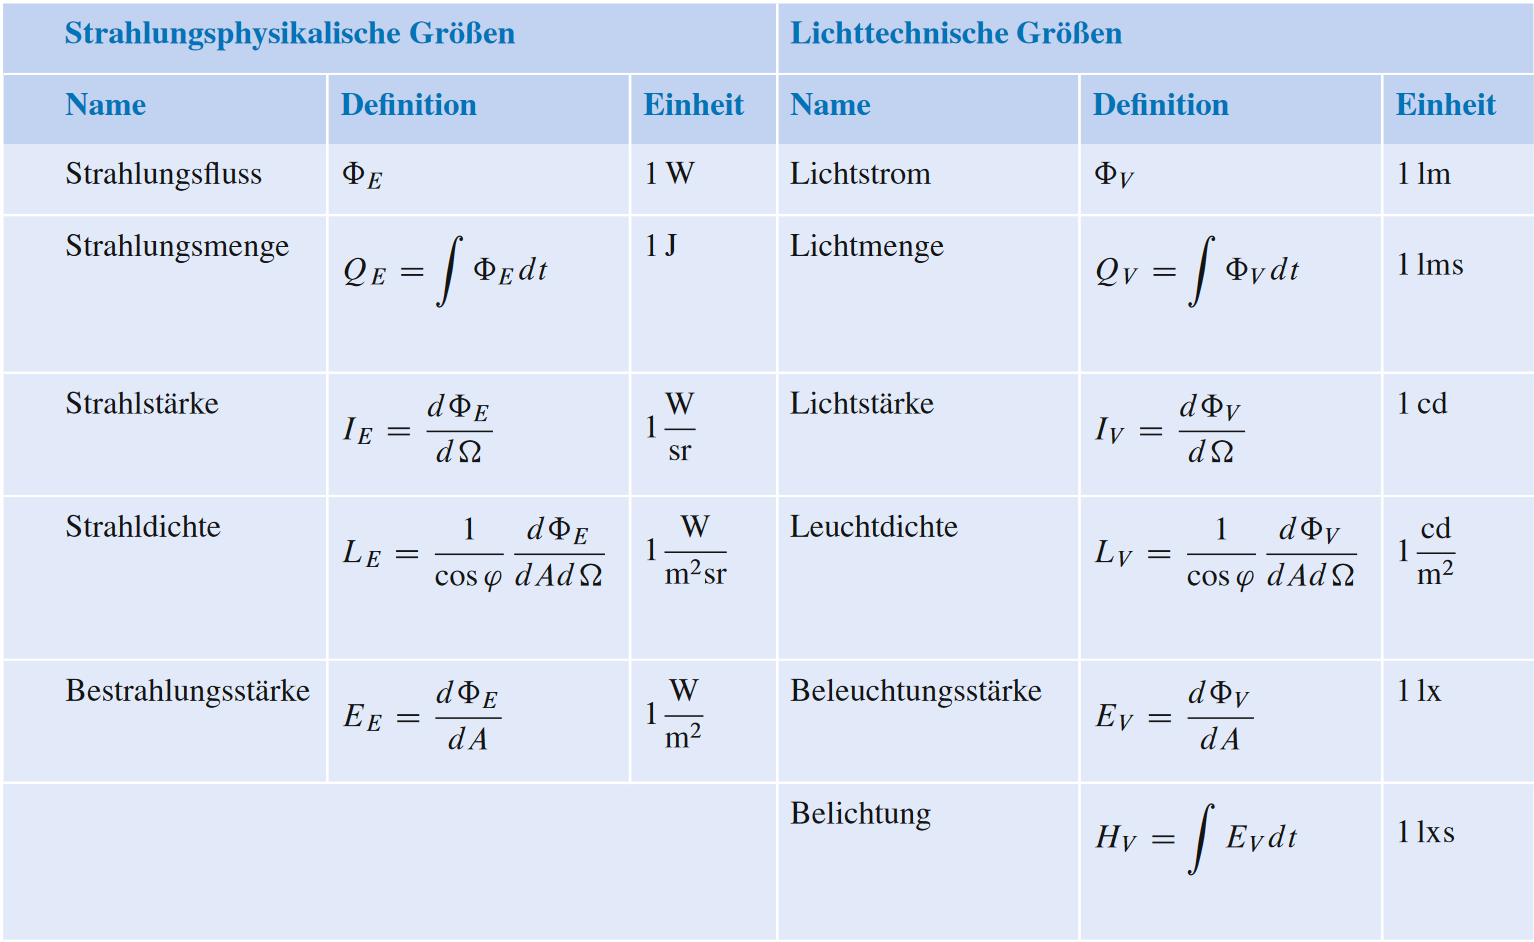
\includegraphics[width=\textwidth]{1.png}
\end{figure}

\begin{lemma}[Stefan-Boltzmann-Gesetz]
    \begin{align*}
        \Phi_E &= \sigma \cdot A \cdot T^4\\
        \sigma &= 5.670 \cdot10^{-8} \ufrac{W}{m^2K^4}\note[Stefan-Boltzmann-Konstante]
    \end{align*}
\end{lemma}

\begin{lemma}[Wien'sches Verschiebungsgesetz]
    Ist \(\lambda_{\te{max}}\) die Wellenlänge, bei der die Emission eines Schwarzerkörpers
    die maximale Intensität zeigt, so gilt:
    \begin{align*}
        \lambda_{max}\cdot T = \const = 2.8978 \E{-3} \mathrm{m\, K}
    \end{align*}
\end{lemma}

\begin{lemma}[Rayleigh-Jean-Gesetz]
    Das Rayleigh-Jean-Gesetz beschreibt die Abstrahlungsleistungspektrum bei hohen Wellenlängen:
    \begin{align*}
        M_E(\lambda):= \frac{\mathrm  d \Phi_E(\lambda)}{\mathrm d\lambda}=2\pi k c\frac T{\lambda^4}
    \end{align*}
\end{lemma}

\begin{lemma}[Wien'sches Strahlungsgesetz]
    Das Wien-Gesetz beschreibt die Abstrahlungsleistungspektrum bei niedrigen Wellenlängen:
    \begin{align*}
        M_E(\lambda) &= \frac{c_1}{\lambda^5} \frac{1}{e^{\frac{c_2}{\lambda T}}}
        = \frac{2\pi h c^2}{\lambda^5} \frac{1}{e^{\frac{h c}{k_B}\frac{1}{\lambda T}}}
    \end{align*}
\end{lemma}
\end{document}